\chapter{Appendix}
\label{appendix}

\section{Combined probability of functions $f$ and $f'$}
\label{apndx:prob}

\hspace{\parindent} The forcing function $f$ permits agents to undergo $\mathrm{R_{1}}$ and is represented with a probability $p_{1}$.
The probability that $\mathrm{R_{1}}$ does not occur is $q_{1} = 1 - p_{1}$.
Likewise for the function $f'$ to undergo $\mathrm{R_{1}}$ is represented with a probability $p_{2}$, and non-occurring probability $q_{2}$.
Combining the probabilities $p$ and $q$ results to

\begin{eqnarray}
\label{eqn:conservP1}
p_{1} + q_{1} &&= 1 \\
\label{eqn:conservP2}
p_{2} + q_{2} &&= 1
\end{eqnarray}

Multiplying the equations \eqref{eqn:conservP1} and \eqref{eqn:conservP2} and simplifying

\begin{eqnarray}
(p_{1} + q_{1})(p_{2} + q_{2}) &&= 1 \\
p_{1}p_{2} + p_{1}q_{2} + p_{2}q_{1} + q_{1}q_{2} &&= 1
\end{eqnarray}

$q_{1}q_{2}$ represents neither event occuring thus

\begin{eqnarray}
p_{net} = 1 - q_{1}q_{2} &&= 1 - (1-p_{1})(1-p_{2}) \\
&&= 1 - (1 - p_{1} - p_{2} + p_{1}p_{2}) \\
&&= p_{1} + p_{2} - p_{1}p_{2}
\label{apndx:simpleProb}
\end{eqnarray}

Replacing \eqref{eq:simpleProb} with the functions gives
\begin{equation}
p_{net} = f + f' - f'f
\end{equation}
which is used in \eqref{eq:p(r1)}

\newpage
\section{Library of applause functions}
\label{apndx:codelib}
\begin{lstlisting}

from random import random
from numpy import zeros, sqrt, sum, nan_to_num
from math import isnan

#function that forces agents to go to state C
def force_func(t, end):
    if t < end:
        return 1
    else:
        return 0

#f'(alpha); feedback based on the number of ppl already in state C; the more ppl in state C, the more ppl will clap
def feedback_alpha(alpha, nC, population):
    return alpha * nC / (population - 1)
    
#g'(beta)
def feedback_beta(beta, nC, population):
    return 1 / (1 + beta * nC / (population - 1))
       
#spatial-dependent feedack, you can control the 'radius' of the reference agent
#taper refers to how many to add at the ends;radius = 0 taper = 1 is '90deg'    
def feedback_space(alpha,system,system_row, system_column, N, M, radius, taper):
    applause_state = []
    for i in range(system_row):
        radius_mech = 0
        applause_state.append(system[i,system_column])
        while radius_mech != radius + taper*(system_row - i):
            radius_mech += 1
            if system_column + radius_mech < M:
                applause_state.append(system[i,system_column + radius_mech])
            if system_column - radius_mech > -1:
                applause_state.append(system[i,system_column - radius_mech])
    return alpha*nan_to_num(sum(applause_state)/len(applause_state))
    
def feedback_180deg(alpha,system,system_row, M): #reverted to simpler feedback space functions since runs took too long
    applause_state = [0]
    for i in range(system_row):
        applause_state.append(sum(system[i]))
    return alpha*nan_to_num(sum(applause_state)/(system_row*M))    

#quadratic equation    
def quad_eq(x,y,z,sign):
    return (-y + sign * (sqrt((y ** 2) - 4 * x * z))) / 2 * x

#do i still need this??!?!
def frange(start, stop, step):
    i = start
    while i < stop:
        yield i
        i += step
   
#creates 'network' of audience        
def audience(N,M,C):
    agents = zeros((N,M))
    
    for i in range(N):
        for j in range(M):
            if sum(agents) == C:
                break
            else:
                agents[i][j]=1
    
    return agents

#the actual simulator            
def app_sim(aStoC, bCtoS, alpha, beta, N, M, C, t, t_1):
    population = N * M
    AGENT = audience(N, M, C)
    graph = []

    for k in range(t):
        nC = sum(AGENT) #number of people clapping
        graph.append(nC)
        for i in range(N):
            for j in range(M):
                if AGENT[i,j] == 0:
                    if random() <= aStoC * (1 - (1-force_func(k, t_1)) * (1 - feedback_alpha(alpha, nC, population))):
                        AGENT[i,j] += 1
                else:
                    if random() <= bCtoS * feedback_beta(beta, nC, population):
                        AGENT[i,j] -= 1
    return graph

#sim with spatial dependence specific to 180 deg
def sim_space(aStoC, bCtoS, alpha, beta, N, M, C, t, t_1):
    population = N * M
    AGENT = audience(N, M, C)
    graph = []
    zeroCount = 0

    for k in range(t):
        nC = sum(AGENT) #number of people clapping
        if nC == 0:
            zeroCount += 1
        graph.append(nC)
        for i in range(N):
            for j in range(M):
                if AGENT[i,j] == 0:
                    if random() <= aStoC * (1 - (1-force_func(k, t_1)) * (1 - feedback_180deg(alpha,AGENT,i, M))):
                        AGENT[i,j] += 1
                else:
                    if random() <= bCtoS * feedback_beta(beta, nC, population):
                        AGENT[i,j] -= 1
        if zeroCount == 6:
            break
            return graph
    return graph
 
#graphs theoretical steady_state based on parameters    
def steady_nC(aStoC, bCtoS, alpha, beta, population, sign):
    if beta == 0:
        if alpha == 0:
            return (aStoC * population) / (aStoC+bCtoS)
        else:
            if sign == 1:
                return population - (bCtoS * (population - 1)) / (aStoC * alpha)
            else:
                return 0
    else:
        if alpha == 0:
            return 0
        else:
            if sign == 0:
                return 0
            else:
                if isnan(quad_eq(1, ((population*aStoC*alpha*beta)-(population*aStoC*alpha)+(aStoC*alpha))/(-aStoC*alpha*beta), (((population**2)*aStoC*alpha) - (population*aStoC*alpha) - ((population**2)*bCtoS) + (2*population*bCtoS) - (bCtoS))/(-aStoC*alpha*beta), sign)) == True:
                    return 0
                else:
                    return quad_eq(1, ((population*aStoC*alpha*beta)-(population*aStoC*alpha)+(aStoC*alpha))/(-aStoC*alpha*beta), (((population**2)*aStoC*alpha) - (population*aStoC*alpha) - ((population**2)*bCtoS) + (2*population*bCtoS) - (bCtoS))/(-aStoC*alpha*beta), sign)

\end{lstlisting}

\newpage
\section{Deriving the steady-state equation}
\label{apndx:derivSS}
\hspace{\parindent} Setting $\frac{d\vec{n}}{dt} = 0$,

\begin{align}
\frac{d}{dt}n_{c} & = 0\\
a(f+f'-f'f)n_{s} - bg'n_{c} & = 0\\
a(f+f'-f'f)n_{s} & = bg'n_{c} \\
\end{align}

Note: $N = n_{c} + n_{s}, n_{s} = N - n{c}$, and $f = 0$.

\begin{equation}
af'(N - n{c}) = bg'n_{c} \\
\label{eq:noFunc}
\end{equation}

Plugging in \eqref{eq:f'} and \eqref{eq:g'} to \eqref{eq:noFunc}:

\begin{align}
a(\alpha\frac{n_{c}}{N-1})(N - n_{c}) &= b(\frac{1}{1 + \frac{\beta n_{c}}{N-1}})(n_{c}) \\
\frac{a\alpha (N - n_{c})}{N-1}n_{c} &= b\frac{N-1}{N-1+\beta n_{c}}n_{c} \\
a\alpha (N - n_{c}) &= b\frac{(N-1)^2}{N-1+\beta n_{c}} \\
a\alpha(N-n_{c})(N-1 + \beta n_{c}) & = b(N-1)^{2}
\end{align}

\newpage
\section{Steady-state Phase Space}
\label{apndx:phaseSpace}
\hspace{\parindent} Shown are the phase space plots for various $b$ values.
\begin{figure}[h!]
 \centering
  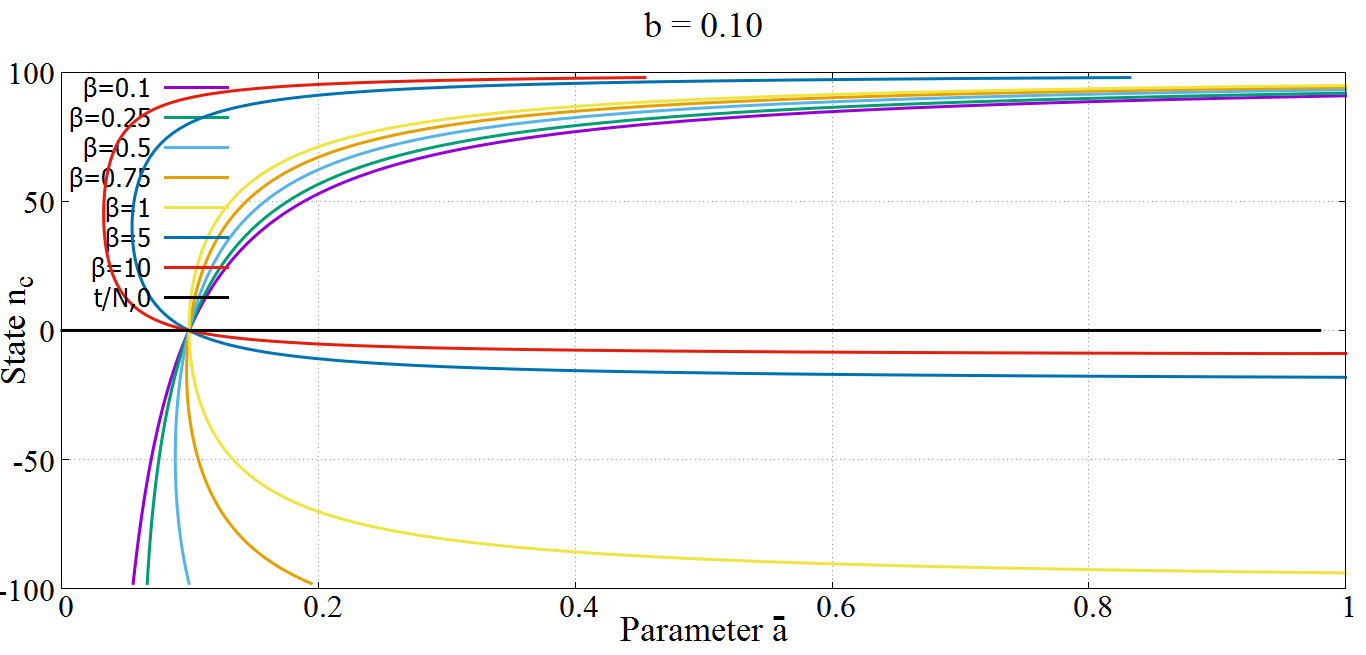
\includegraphics[width=\linewidth]{images/appendix/phaseSpace/1.png}
\end{figure}

\begin{figure}[h!]
 \centering
  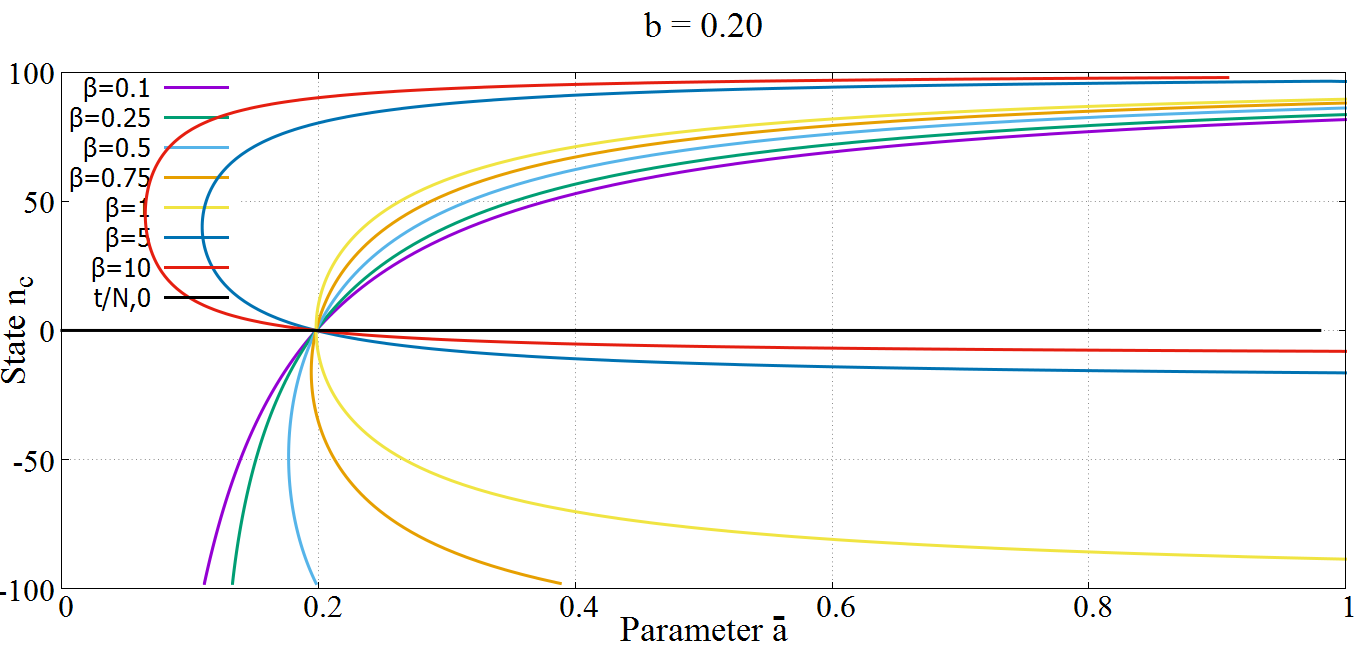
\includegraphics[width=\linewidth]{images/appendix/phaseSpace/2.png}
\end{figure}

\begin{figure}[h!]
 \centering
  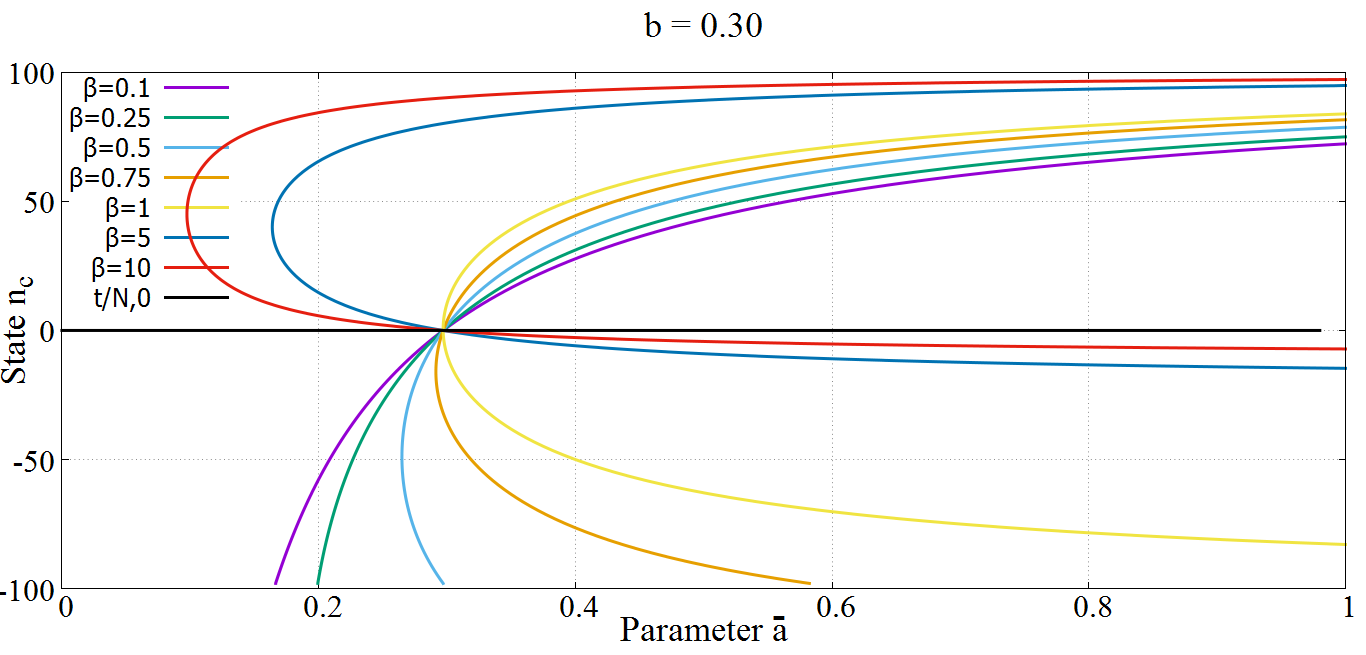
\includegraphics[width=\linewidth]{images/appendix/phaseSpace/3.png}
\end{figure}
\newpage
\begin{figure}[h!]
 \centering
  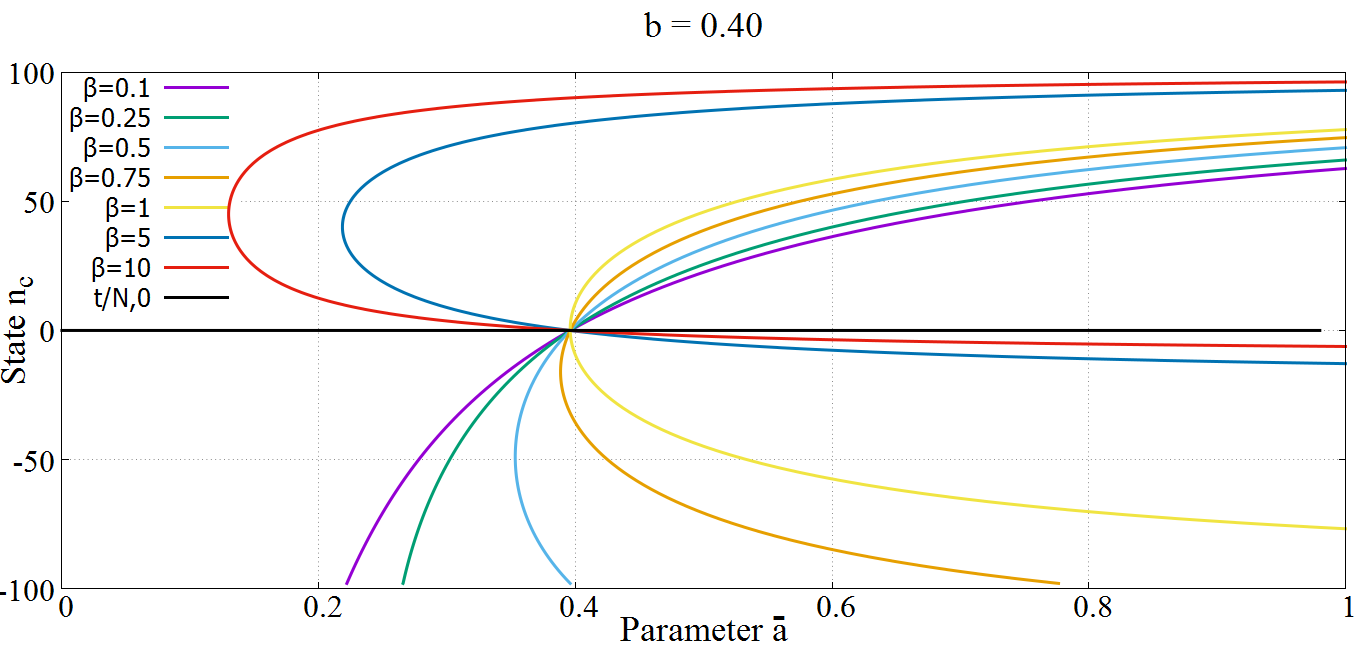
\includegraphics[width=\linewidth]{images/appendix/phaseSpace/4.png}
\end{figure}
\newpage
\begin{figure}[h!]
 \centering
  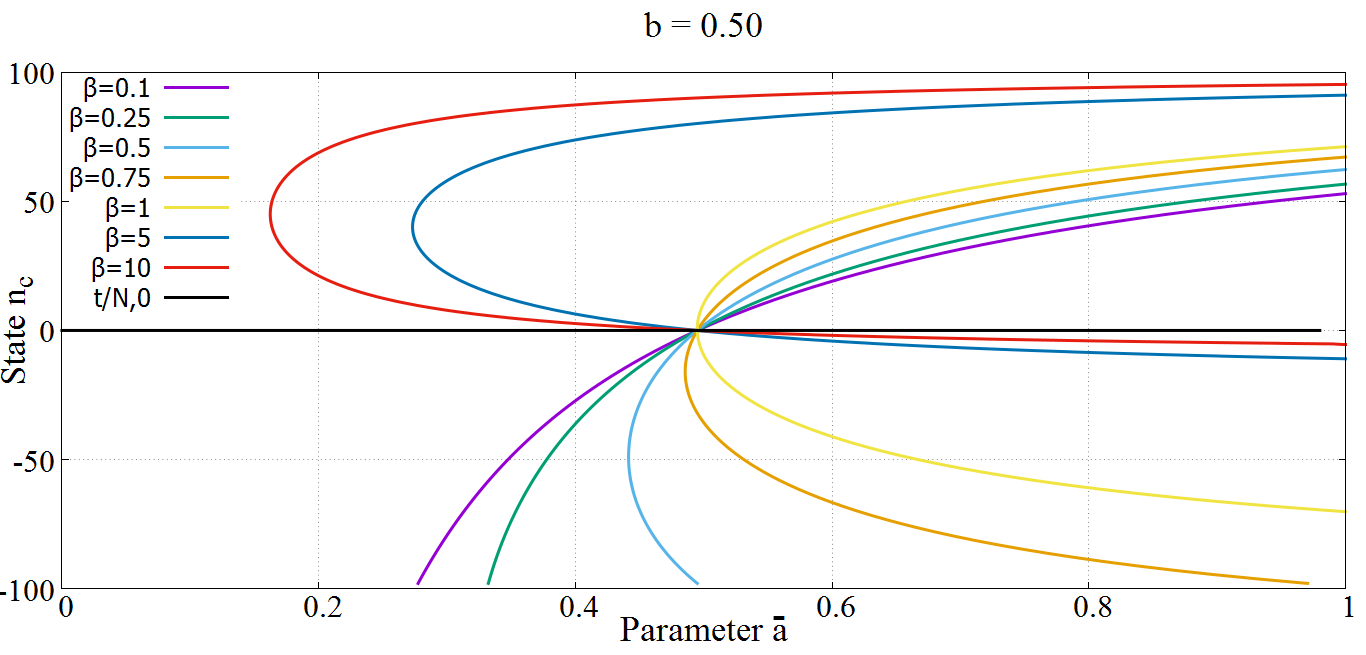
\includegraphics[width=\linewidth]{images/appendix/phaseSpace/5.png}
\end{figure}

\begin{figure}[h!]
 \centering
  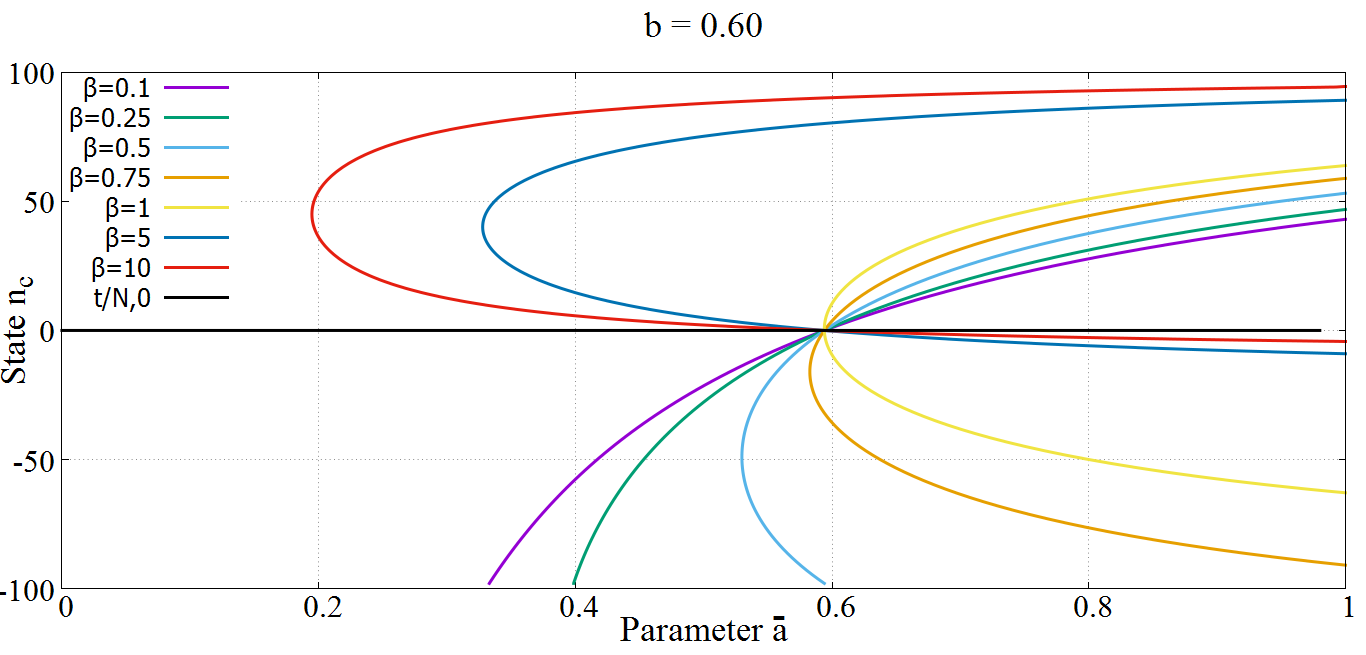
\includegraphics[width=\linewidth]{images/appendix/phaseSpace/6.png}
\end{figure}
\newpage
\begin{figure}[h!]
 \centering
  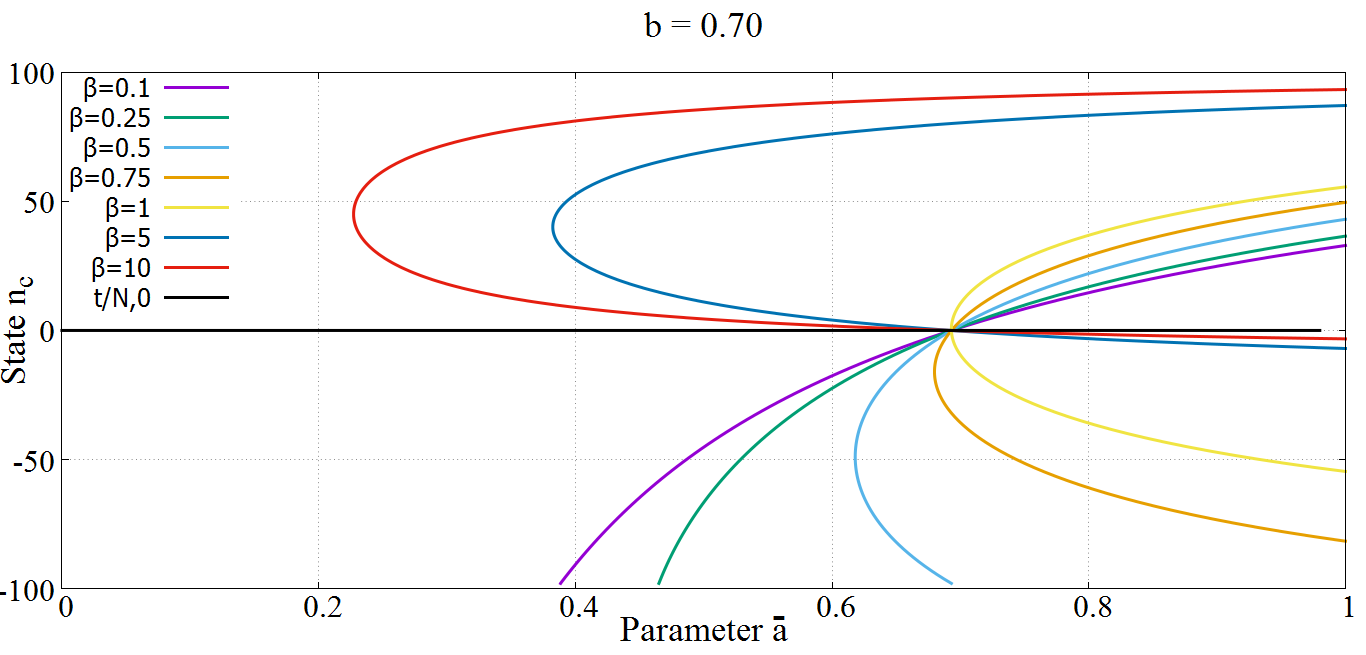
\includegraphics[width=\linewidth]{images/appendix/phaseSpace/7.png}
\end{figure}

\begin{figure}[h!]
 \centering
  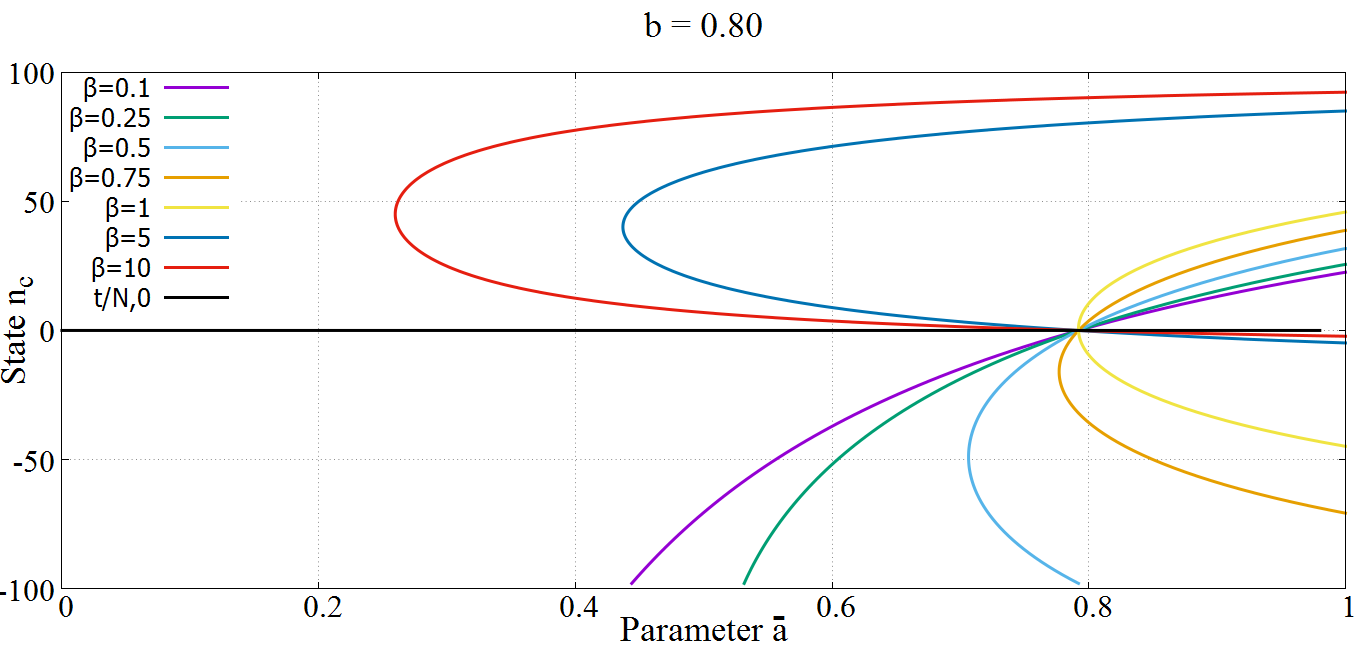
\includegraphics[width=\linewidth]{images/appendix/phaseSpace/8.png}
\end{figure}
\newpage
\begin{figure}[h!]
 \centering
  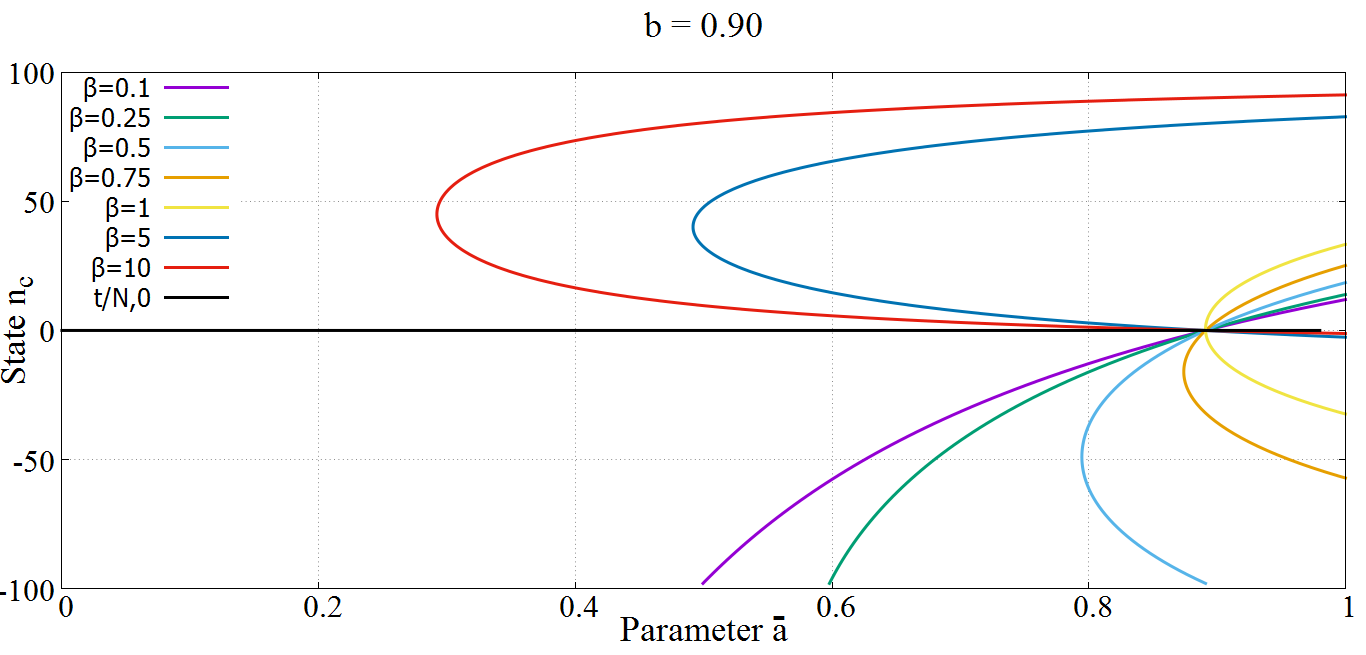
\includegraphics[width=\linewidth]{images/appendix/phaseSpace/9.png}
\end{figure}

\begin{figure}[h!]
 \centering
  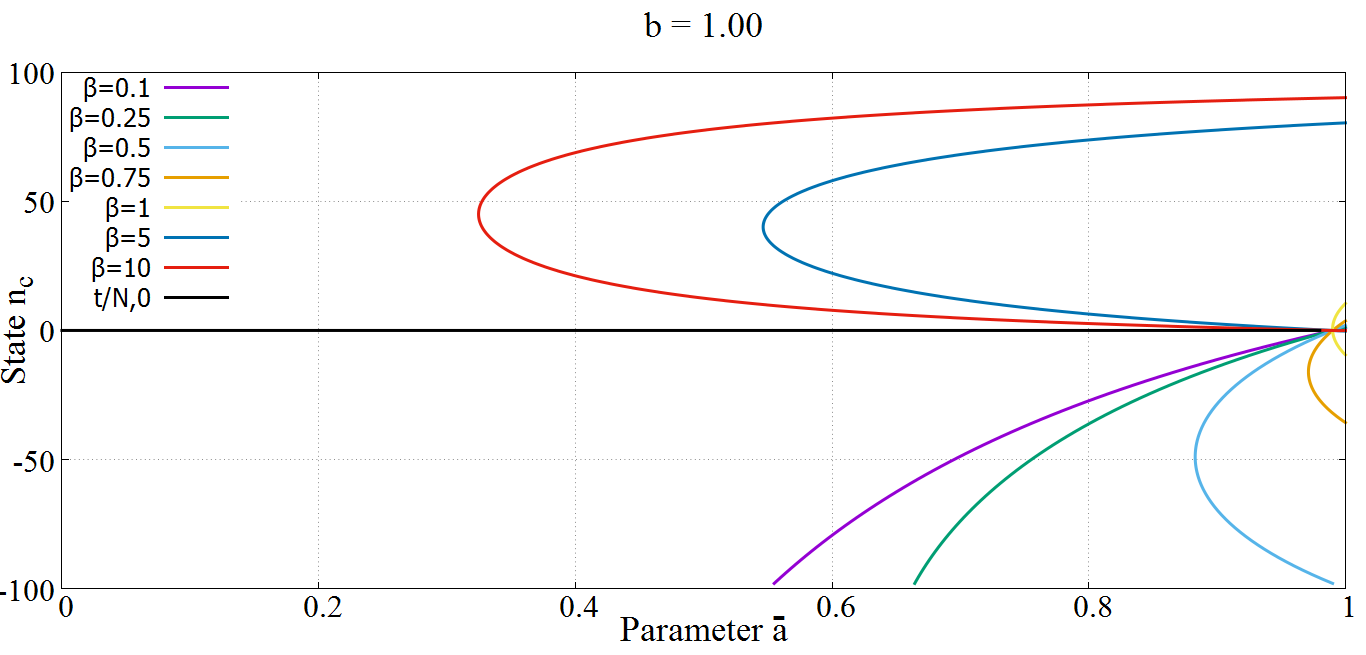
\includegraphics[width=\linewidth]{images/appendix/phaseSpace/10.png}
\end{figure}

\newpage
\section{Critical points}
\label{apndx:crita1}
\hspace{\parindent} Setting $n_{c} = 0$ in the steady-state equation \eqref{eq:steadystate} gives us this critical point of intersection

\begin{eqnarray}
\bar{a}(N-n_{c})(N-1 + \beta n_{c}) &&= b(N-1)^{2} \\
\bar{a}N(N-1) &&= b(N-1)^{2} \\
\bar{a} &&= \frac{b(N-1)^{2}}{N(N-1)} \\
\bar{a}_{1} &&= \frac{b(N-1)}{N} \\
\end{eqnarray}

On the other hand, $\bar{a_{2}}$ is arrived by plugging in a special $n_{c}$ value, $n_{c}^{*} \equiv [1+(\beta-1)N]/2\beta$.

\begin{eqnarray}
\bar{a}(N-n_{c}^{*})(N-1 + \beta n_{c}^{*}) &&= b(N-1)^{2} \\
\bar{a}_{2} &&= \frac{b(N-1)^{2}}{(N-n_{c}^{*})(N-1 + \beta n_{c}^{*})}
\end{eqnarray}

\newpage
\section{Steady-state Simulations}
\label{apndx:steadstatesim}
Shown is the code that outputs the simulations with the analytical steady-state as well as the mean of the system for a single set of parameters.

\begin{lstlisting}

#####################################################
#Simulates applause for a specific set of parameters#
#Displays the appropriate steady state value        #
#Parameters can be adjusted accordingly below       #
#####################################################


import applause_functions as app
import matplotlib.pyplot as plt
import numpy as np

N = 10
M = 10
population = N * M
time = 500
t_1 = 2
C = 0
aStoC = 1
bCtoS = 0.8
alpha = 0.6
beta = 1

fig = plt.figure()
ax = fig.add_subplot(111)
sim = app.app_sim(aStoC, bCtoS, alpha, beta, N, M, C, time, t_1)
plt.plot(sim)
ax.text(0.45*time,1,'Steady-state:'+str(round(app.steady_nC(aStoC, bCtoS, alpha, beta, population, 1),0)), fontsize=20)
ax.text(0.45*time,10,'Mean: '+str(round(np.mean(sim),1))+'$\pm$'+str(round(np.std(sim),2)), fontsize=20)
ax.text(10,100,'N = '+str(population), fontsize=15)
plt.axhline(np.mean(sim), color = 'r')
plt.axhline(app.steady_nC(aStoC, bCtoS, alpha, beta, population, 1), color = 'g')
plt.title('$a = $'+str(aStoC)+' $b = $'+str(bCtoS)+r' $\alpha=$'+str(alpha)+r' $\beta=$'+str(beta),fontsize=20)
plt.xlabel('Time',fontsize=18)
plt.ylabel('State'+r' $n_{c}$',fontsize=18)
plt.xlim(0,time)
plt.ylim(0,110)
plt.savefig('ssB.png')
plt.show()

\end{lstlisting}

Following is the code used to generate the data points of the simulated steady-state values to be plotted against the analytic steady-state solutions.

\begin{lstlisting}

#Takes the last point of the simulation (Trials) times then calculates mean and std#
#Does so for varying a-bar values                                                  #
#Creates .csv file with columns: a-bar, mean, std                                  #
#Plots the data points                                                             #
#Parameters can be adjusted accordingly below                                      #


import applause_functions as app
import matplotlib.pyplot as plt
import numpy as np

#####Simulation Parameters#####
N = 10
M = 10
startPop = 20
time = 100
t_1 = 0
aStoC = 1.0
bCtoS = 0.8 
alpha = 1
beta = 10
###Point Generator Parameters###
Trials = 50
interval = 0.02
##############################
def pointGen(aStoC, bCtoS, beta, N, M, startPop, time, t_1, Trials, interval):
    
    meanlist = []
    stdlist = []
    ilist = []
    for i in np.arange(0,1.0,interval):
        list_a = []
        for j in range(Trials):
            list_a.append(app.app_sim(aStoC, bCtoS, i, beta, N, M, startPop, time, t_1)[time-1]) #takes the last number from the appsim vector
        mean = np.mean(np.array(list_a))
        std = np.std(np.array(list_a))  
        meanlist.append(mean)
        stdlist.append(std)
        ilist.append(i)

    ilist = np.array(ilist)
    meanlist = np.array(meanlist)
    stdlist = np.array(stdlist)
    
    #writes ilist,meanlist, and stdlist into a txt file
    filename = 'b = ' + str(bCtoS) + ', beta = ' + str(beta) + ', startPop = ' + str(startPop) + '.txt'    
    with open(filename,'w') as f:
        lis=[ilist,meanlist,stdlist]
        for x in zip(*lis):
            f.write("{0}\t{1}\t{2}\n".format(*x))
            
    return (ilist,meanlist,stdlist)
\end{lstlisting}

\newpage
\section{Steady-state Simulations Results}
\label{apndx:ssexpt}
Shown are the phase space plots along with the simulated data points using the same parameters for various $b$ and $\beta$ values.

\begin{figure}[h!]
 \centering
  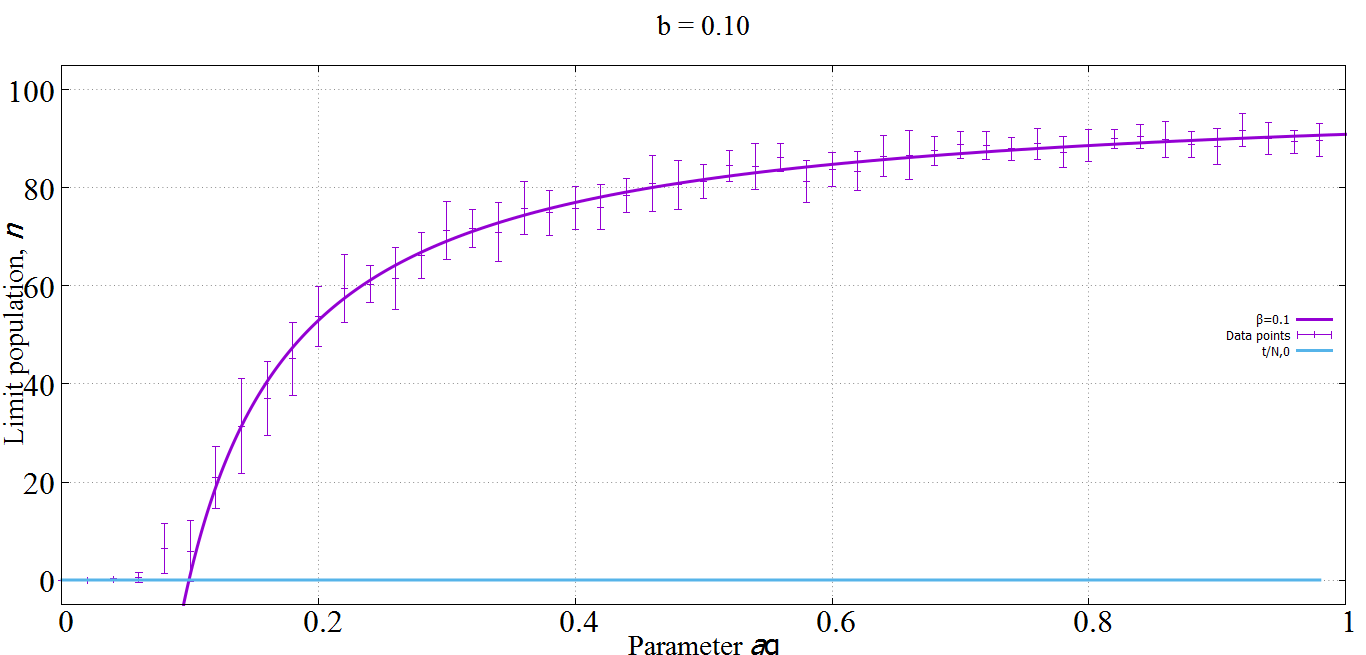
\includegraphics[width=\linewidth]{images/appendix/simexpt/1.png}
\end{figure}

\begin{figure}[h!]
 \centering
  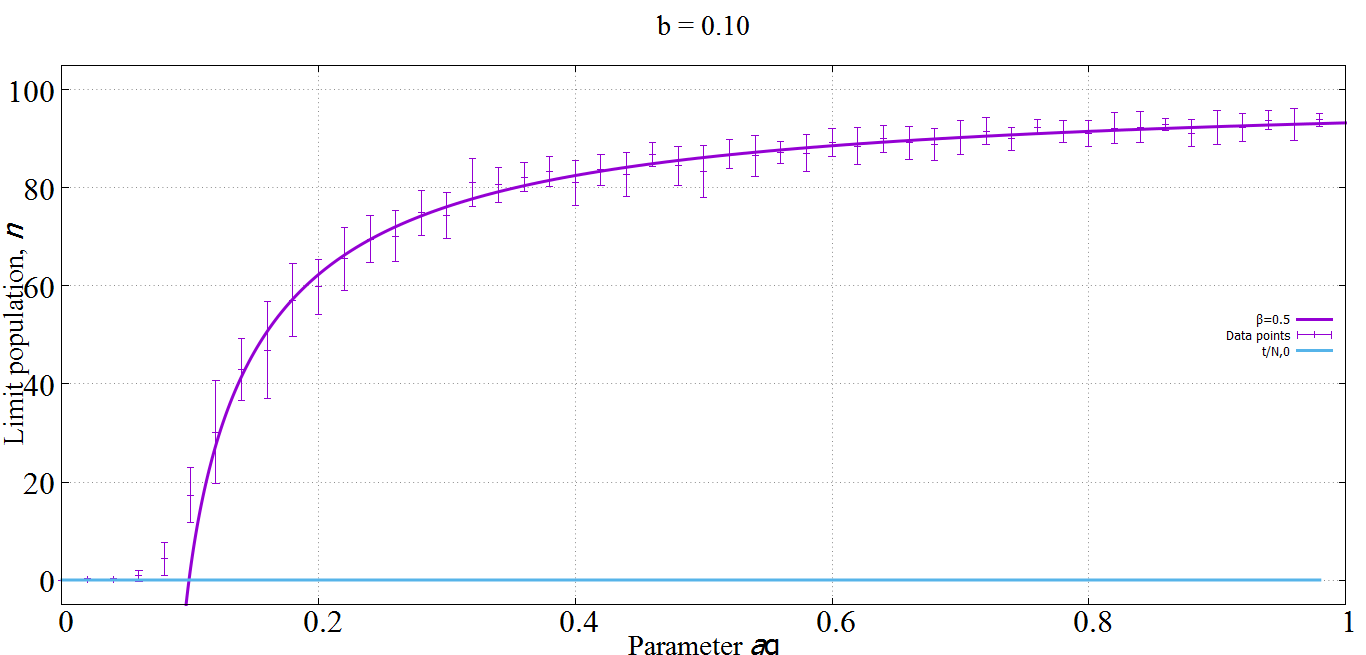
\includegraphics[width=\linewidth]{images/appendix/simexpt/2.png}
\end{figure}
\newpage
\begin{figure}[h!]
 \centering
  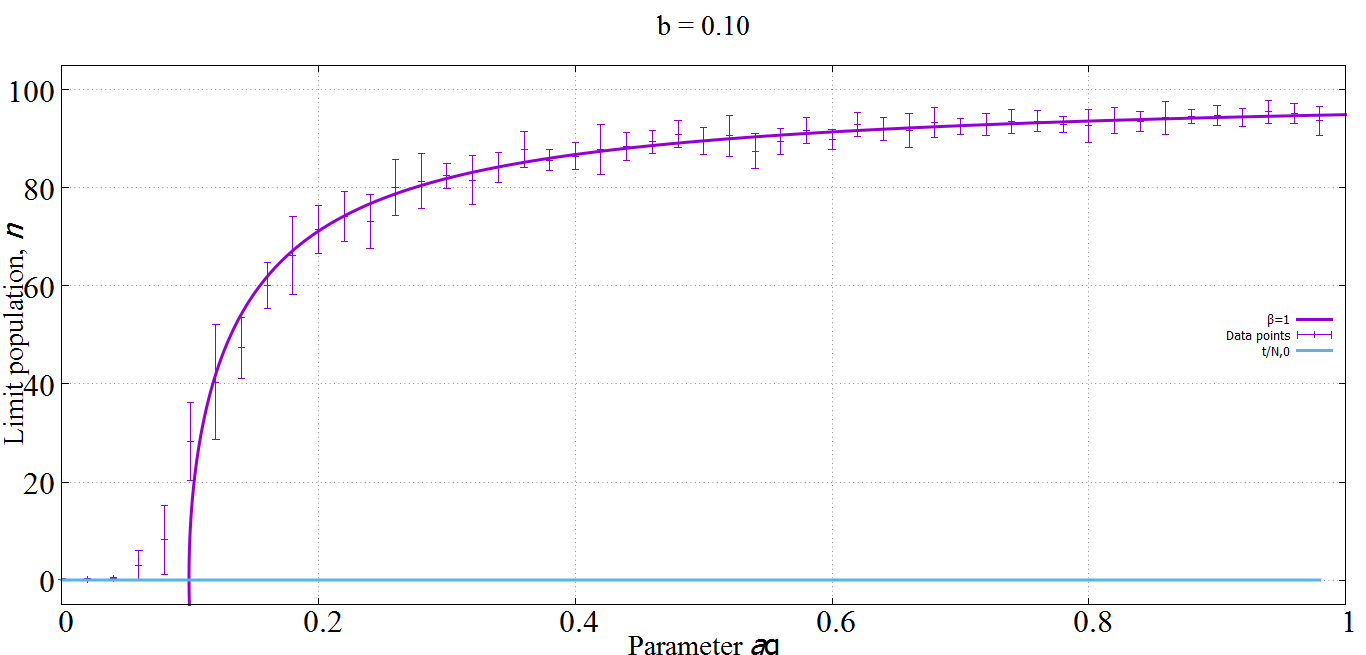
\includegraphics[width=\linewidth]{images/appendix/simexpt/3.png}
\end{figure}

\begin{figure}[h!]
 \centering
  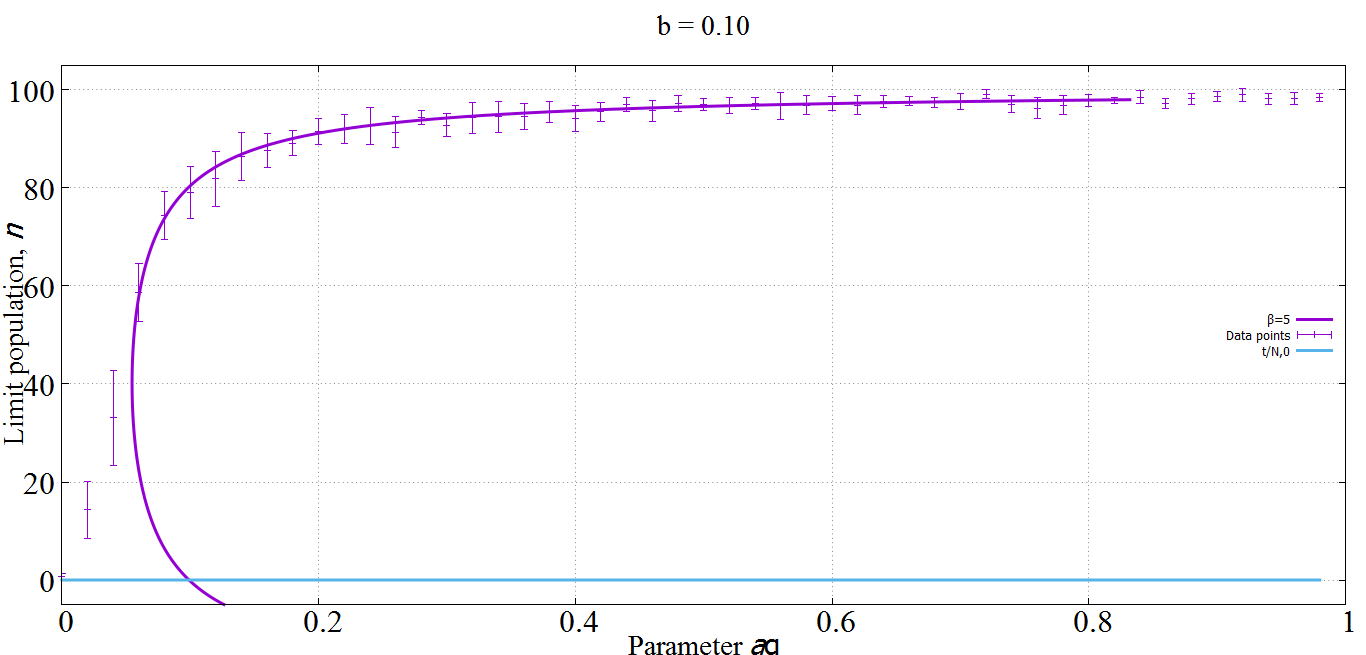
\includegraphics[width=\linewidth]{images/appendix/simexpt/4.png}
\end{figure}
\newpage
\begin{figure}[h!]
 \centering
  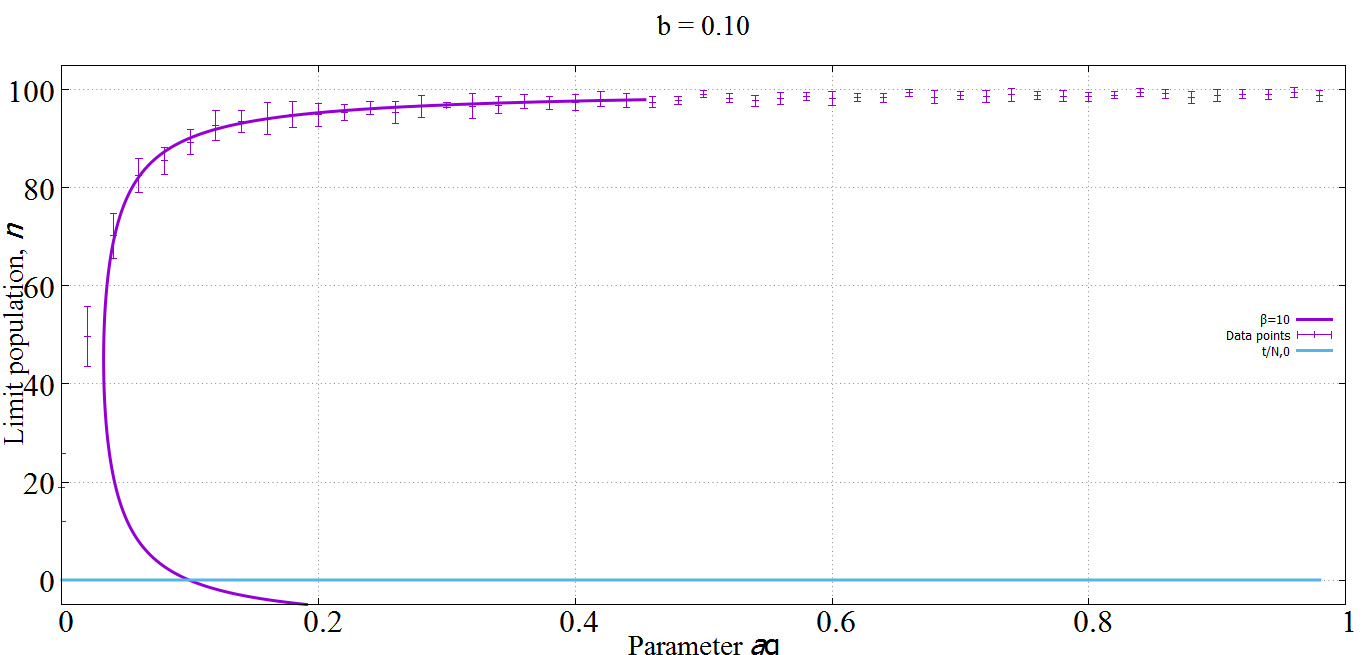
\includegraphics[width=\linewidth]{images/appendix/simexpt/5.png}
\end{figure}

\begin{figure}[h!]
 \centering
  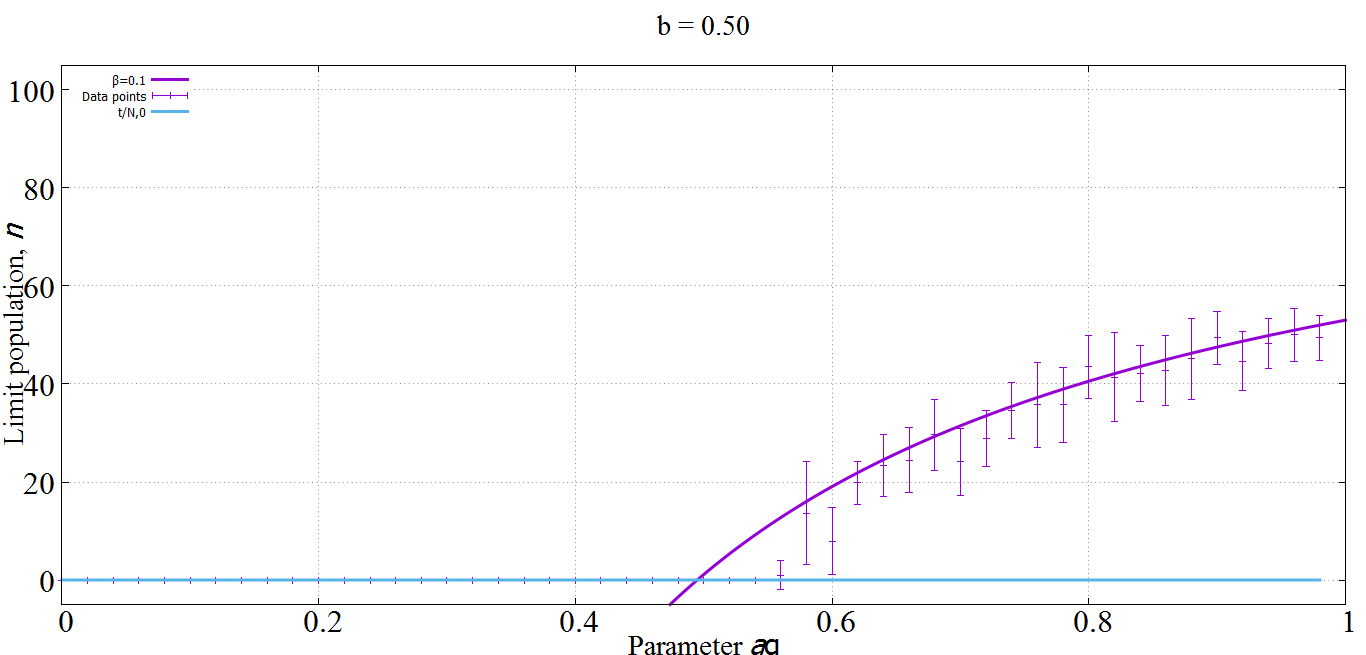
\includegraphics[width=\linewidth]{images/appendix/simexpt/6.png}
\end{figure}
\newpage
\begin{figure}[h!]
 \centering
  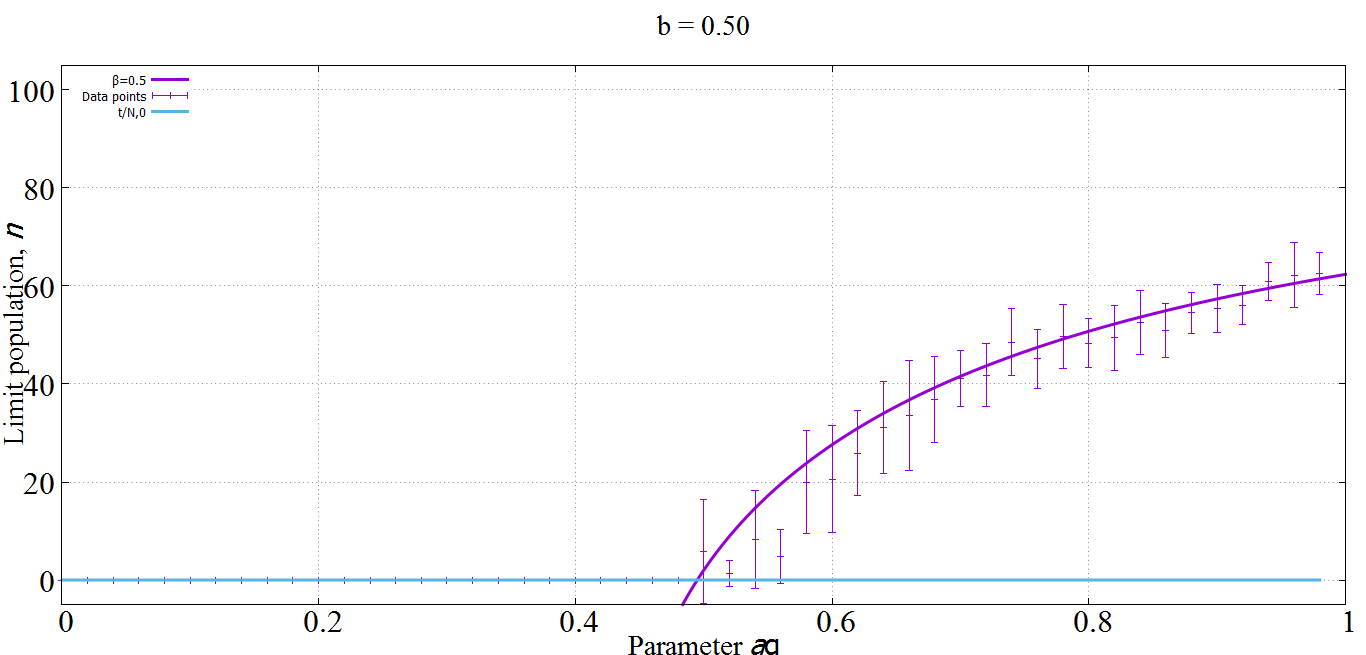
\includegraphics[width=\linewidth]{images/appendix/simexpt/7.png}
\end{figure}

\begin{figure}[h!]
 \centering
  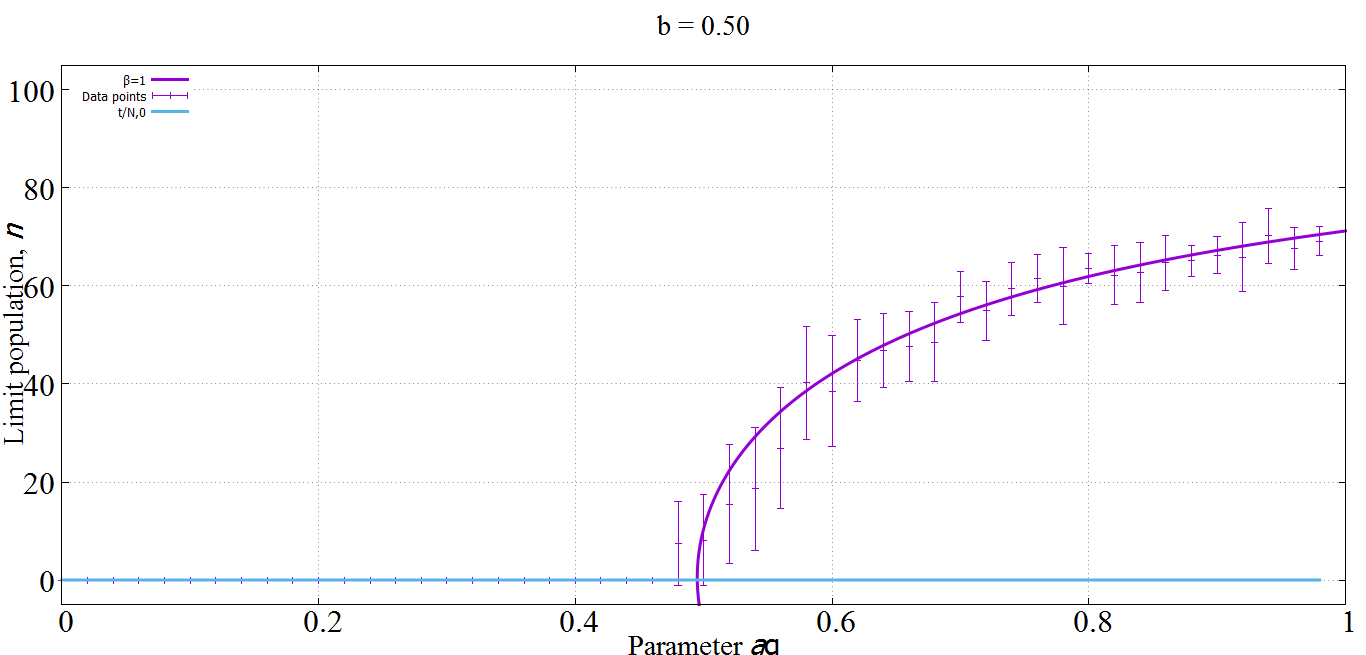
\includegraphics[width=\linewidth]{images/appendix/simexpt/8.png}
\end{figure}
\newpage
\begin{figure}[h!]
 \centering
  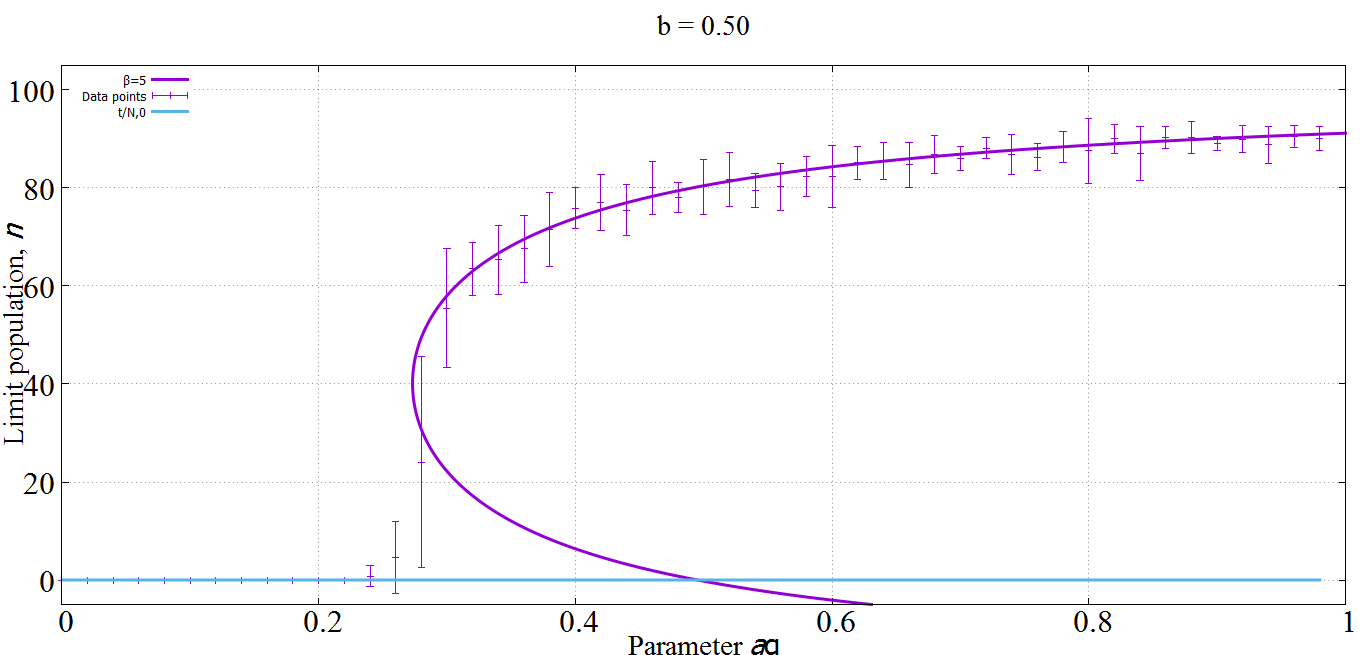
\includegraphics[width=\linewidth]{images/appendix/simexpt/9.png}
\end{figure}

\begin{figure}[h!]
 \centering
  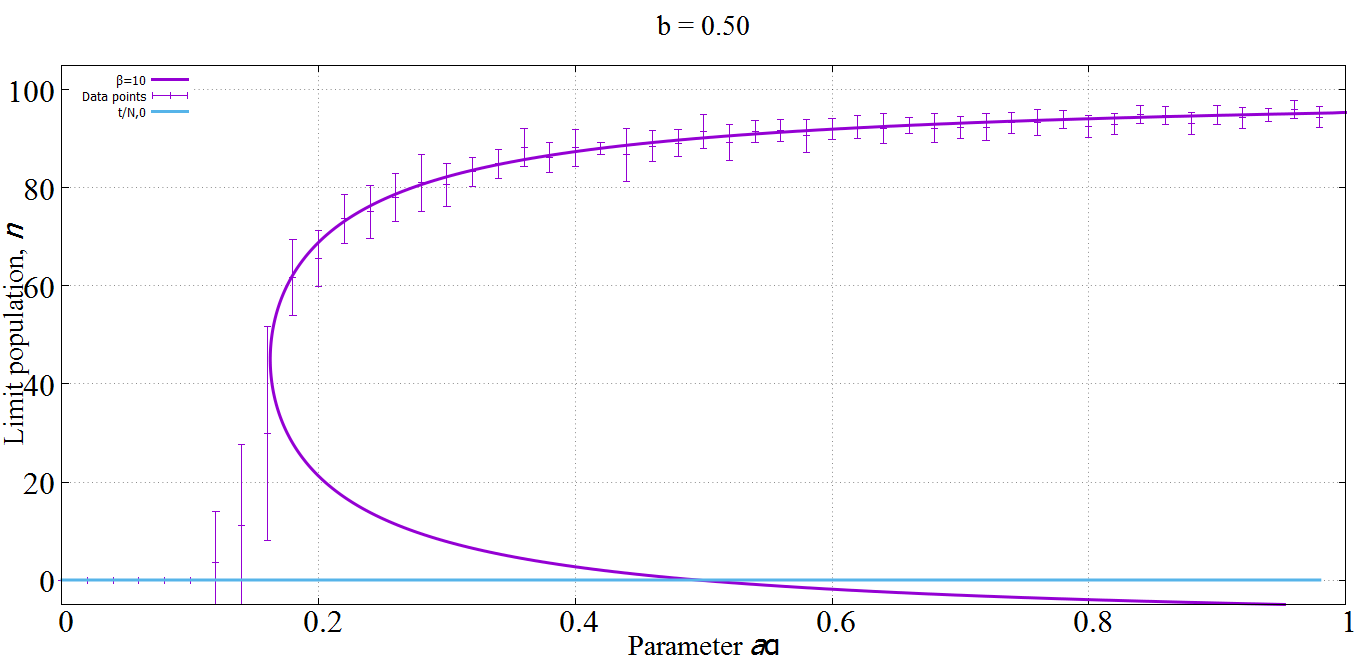
\includegraphics[width=\linewidth]{images/appendix/simexpt/10.png}
\end{figure}
\newpage
\begin{figure}[h!]
 \centering
  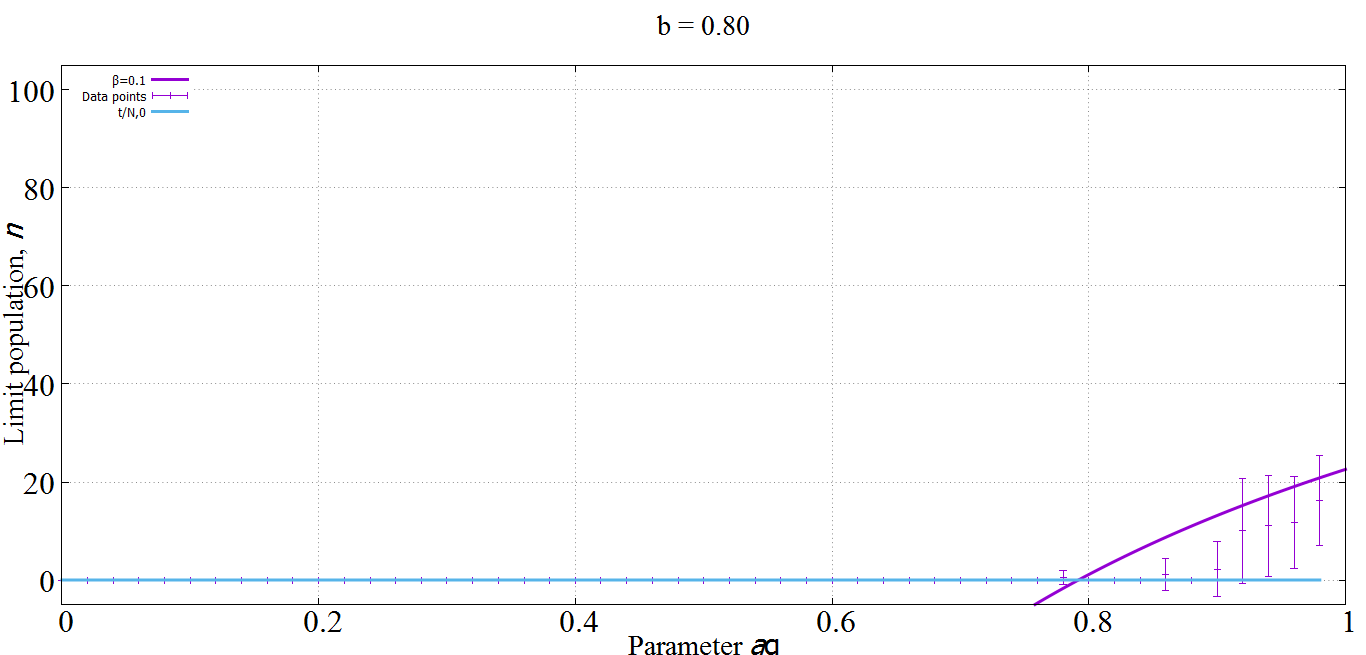
\includegraphics[width=0.6\linewidth]{images/appendix/simexpt/11.png}
\end{figure}

\begin{figure}[h!]
 \centering
  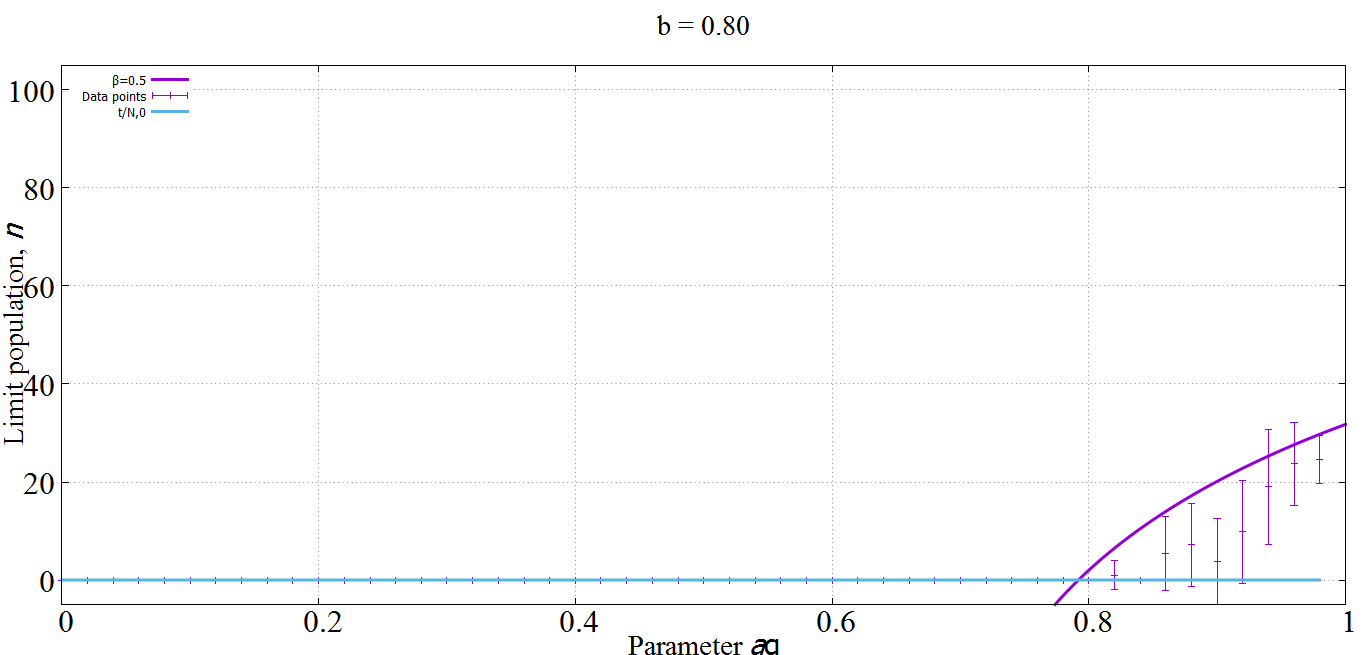
\includegraphics[width=0.6\linewidth]{images/appendix/simexpt/12.png}
\end{figure}

\begin{figure}[h!]
 \centering
  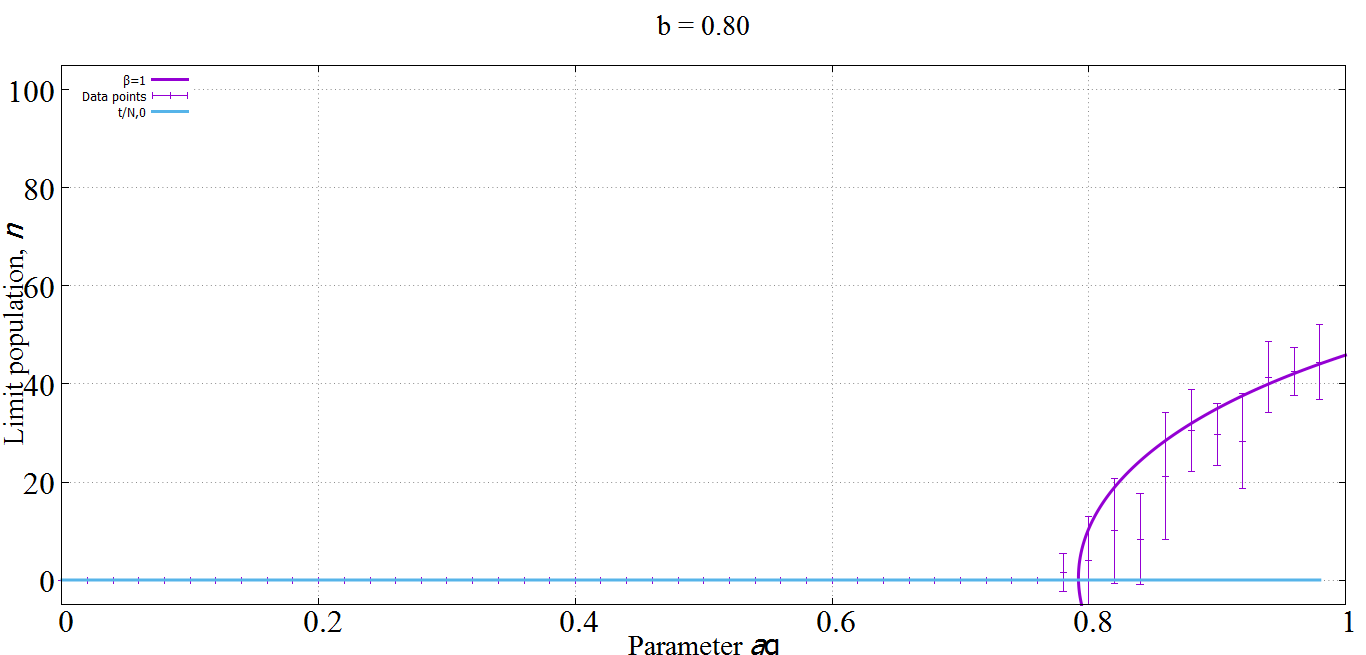
\includegraphics[width=0.6\linewidth]{images/appendix/simexpt/13.png}
\end{figure}
\newpage
\begin{figure}[h!]
 \centering
  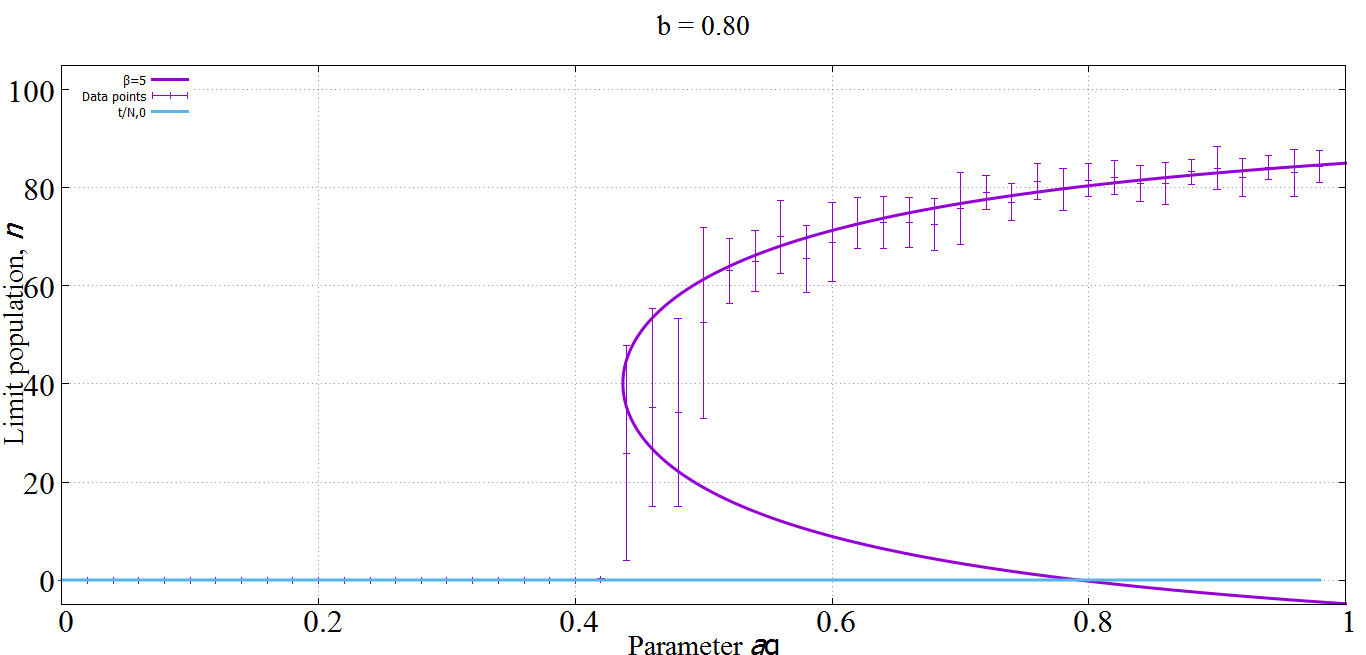
\includegraphics[width=\linewidth]{images/appendix/simexpt/14.png}
\end{figure}

\begin{figure}[h!]
 \centering
  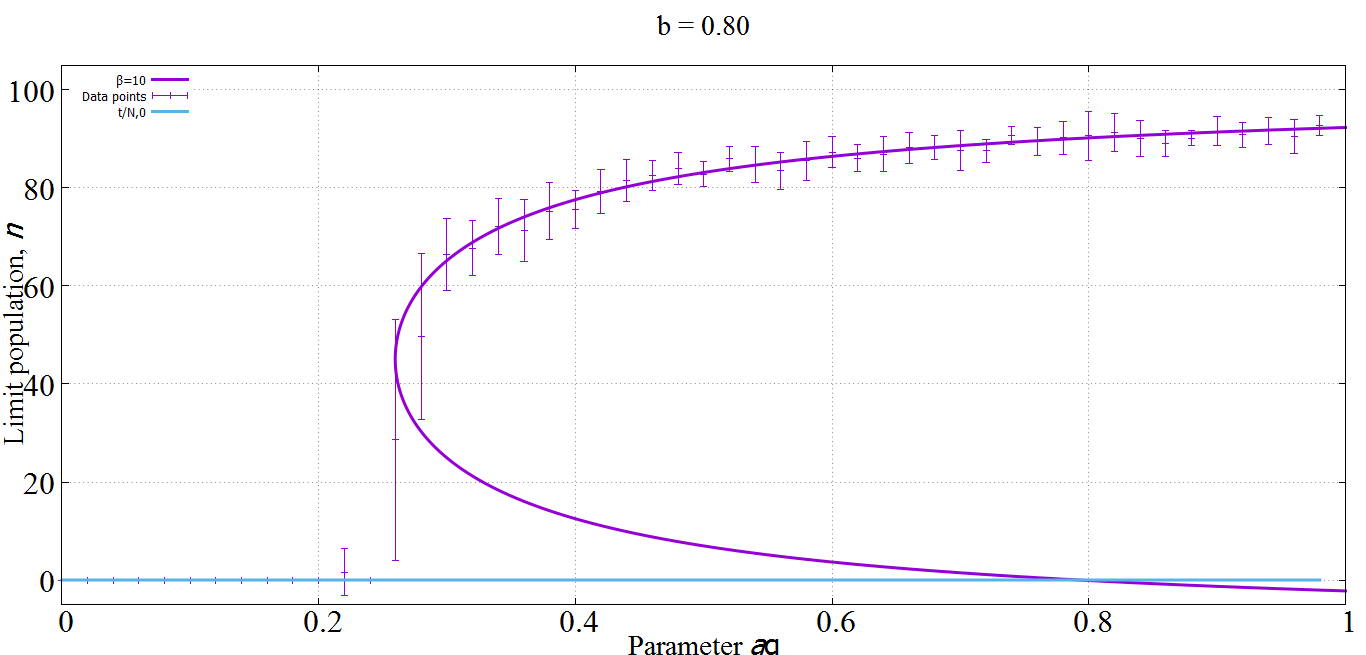
\includegraphics[width=\linewidth]{images/appendix/simexpt/15.png}
\end{figure}

\newpage
\section{Vector Generator}
\label{apndx:vectsim}

Following is the code used to generate the vectors pointing to the steady-state given the initial to be plotted against the analytic steady-state solutions.

\begin{lstlisting}
import applause_functions as app
import matplotlib.pyplot as plt
import numpy as np
import time as t

speed = t.clock()

N = 10
M = 10
startPop = 1
time = 100
t_1 = 0
aStoC = 1.0
bCtoS = 0.8 
alpha = 1
beta = 10

x = 11
y = 11
z = 100

#a = app.app_sim(aStoC, bCtoS, alpha, beta, N, M, startPop, time, t_1)

def probFilter(a): #converts all non-zero values in a list to 1
    for q in range(len(a)):
        if a[q] != 0:
            a[q] = 1

def lastList(abar, bCtoS, alpha, beta, N, M, start, time, t_1, iter): 
    #runs app_sim 'iter' times and lists the last element per iteration
    finalVal = []
    probVal = []
    for i in range(iter):
        x = app.app_sim(abar, bCtoS, alpha, beta, N, M, start, time, t_1)[-1]
        finalVal.append(x)
        if x==0:
            probVal.append(0.0)
        else:
            probVal.append(1.0)
    return finalVal, probVal
    
    
def heatData(bCtoS, beta, x, y, z):
    abarRange = np.linspace(0,1,x)
    startRange = np.linspace(0,100,y)  
    
    n = 0
    
    abar = np.zeros(len(abarRange)*len(startRange))
    start = np.zeros(len(abarRange)*len(startRange))
    rawHeat = np.zeros(len(abarRange)*len(startRange))
        
    for i in range(len(abarRange)):
        for j in range(len(startRange)):
            k = lastList(abarRange[i], bCtoS, alpha, beta, N, M, startRange[j], time, t_1, z)
            abar[n] = (abarRange[i])
            start[n] = (startRange[j])
            rawHeat[n] =(sum(k[1])/len(k[1]))
            n += 1
            print(t.clock() - speed)
            
    
    filename = 'b = ' + str(bCtoS) + ', beta = ' + str(beta) + ', x = ' + str(x) + ', y = ' + str(y) + ', z = ' + str(z) + '.txt'    
    with open(filename,'w') as f:
        lis=[abar,start,rawHeat]
        for x in zip(*lis):
            f.write("{0}\t{1}\t{2}\n".format(*x))        
            
    return abar,start,rawHeat
\end{lstlisting}

\newpage
\section{Vector Graphs}
\label{apndx:vectgraph}
Shown are the phase space plots along with probabilistic vectors pointing towards the steady-state for various $b$ and $\beta$ values.

\begin{figure}[h!]
 \centering
  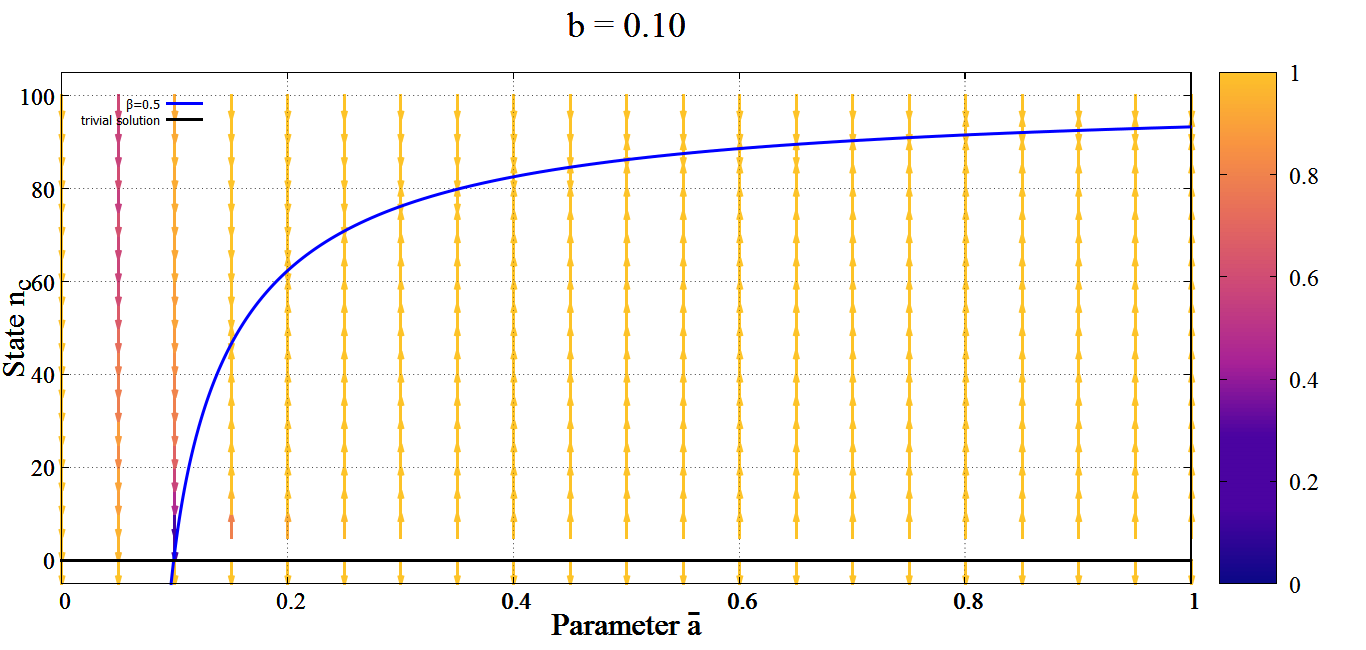
\includegraphics[width=\linewidth]{images/appendix/vectors/1.png}
\end{figure}

\begin{figure}[h!]
 \centering
  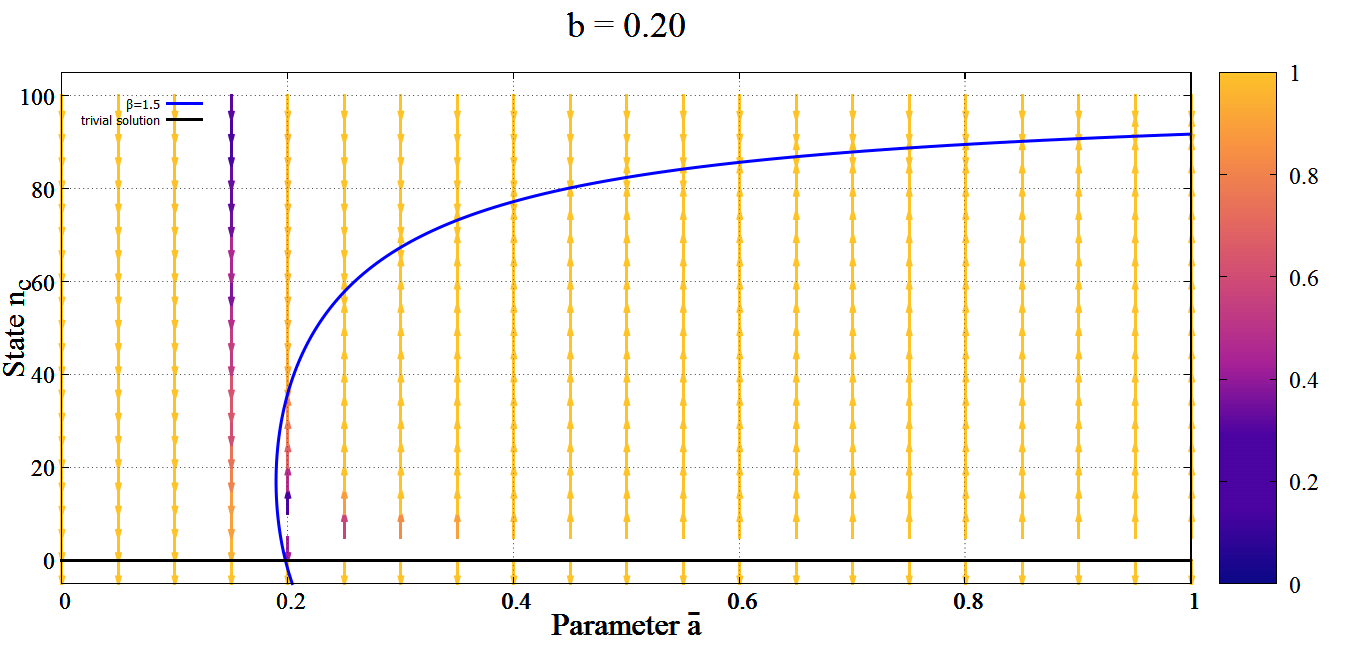
\includegraphics[width=\linewidth]{images/appendix/vectors/2.png}
\end{figure}
\newpage
\begin{figure}[h!]
 \centering
  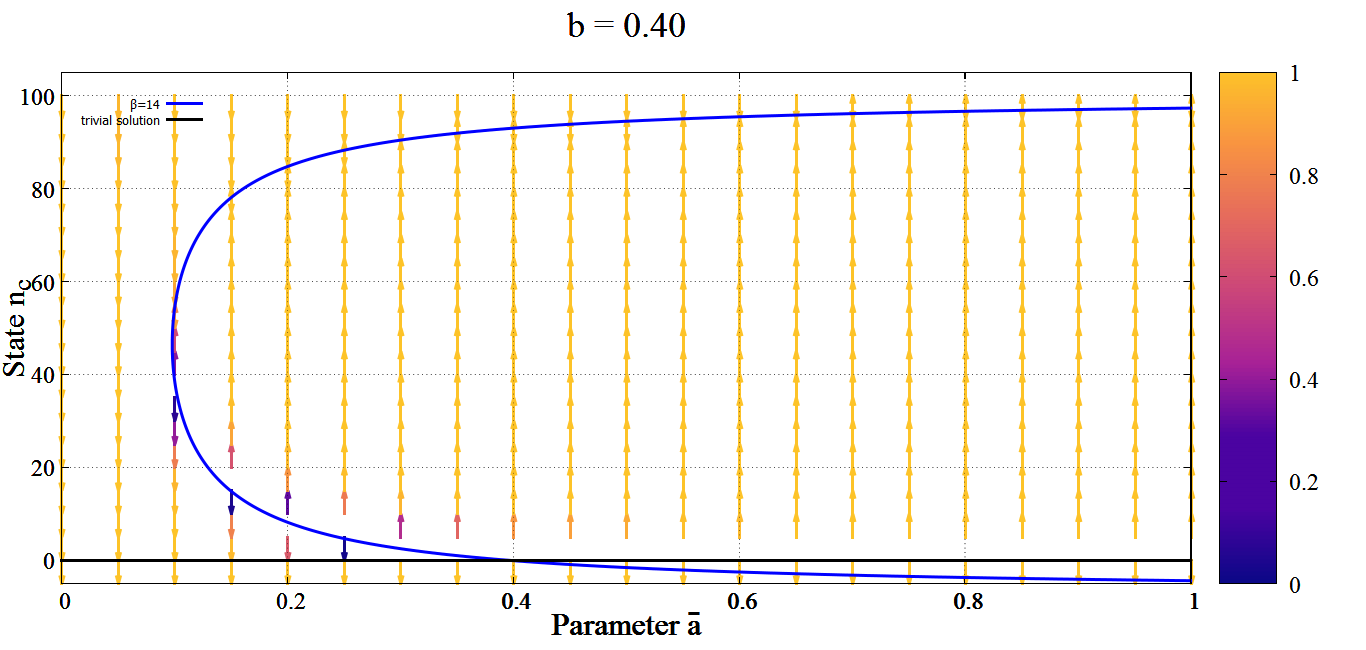
\includegraphics[width=\linewidth]{images/appendix/vectors/3.png}
\end{figure}

\begin{figure}[h!]
 \centering
  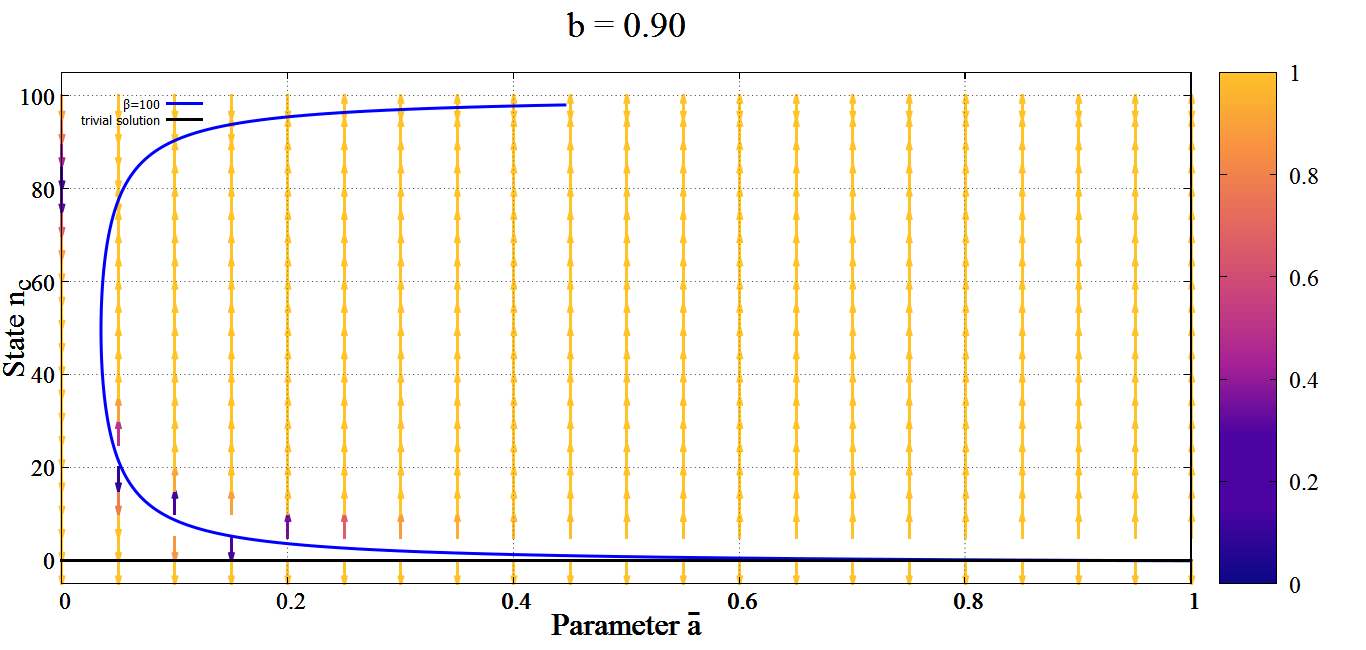
\includegraphics[width=\linewidth]{images/appendix/vectors/5.png}
\end{figure}

\newpage
\section{asdf}
\label{apndx:asdf}